\documentclass[12pt,a4paper]{report}
\usepackage[utf8]{inputenc}
\usepackage[russian]{babel}
\usepackage[OT1]{fontenc}
\usepackage{amsmath}
\usepackage{amsfonts}
\usepackage{amssymb}
\usepackage{graphicx}
\usepackage{cmap}					% поиск в PDF
\usepackage{mathtext} 				% русские буквы в формулах
%\usepackage{tikz-uml}               % uml диаграммы

% TODOs
\usepackage[%
  colorinlistoftodos,
  shadow
]{todonotes}

% Генератор текста
\usepackage{blindtext}

%------------------------------------------------------------------------------

% Подсветка синтаксиса
\usepackage{color}
\usepackage{xcolor}
\usepackage{listings}
 
 % Цвета для кода
\definecolor{string}{HTML}{B40000} % цвет строк в коде
\definecolor{comment}{HTML}{008000} % цвет комментариев в коде
\definecolor{keyword}{HTML}{1A00FF} % цвет ключевых слов в коде
\definecolor{morecomment}{HTML}{8000FF} % цвет include и других элементов в коде
\definecolor{captiontext}{HTML}{FFFFFF} % цвет текста заголовка в коде
\definecolor{captionbk}{HTML}{999999} % цвет фона заголовка в коде
\definecolor{bk}{HTML}{FFFFFF} % цвет фона в коде
\definecolor{frame}{HTML}{999999} % цвет рамки в коде
\definecolor{brackets}{HTML}{B40000} % цвет скобок в коде
 
 % Настройки отображения кода
\lstset{
language=C, % Язык кода по умолчанию
morekeywords={*,...}, % если хотите добавить ключевые слова, то добавляйте
 % Цвета
keywordstyle=\color{keyword}\ttfamily\bfseries,
stringstyle=\color{string}\ttfamily,
commentstyle=\color{comment}\ttfamily\itshape,
morecomment=[l][\color{morecomment}]{\#}, 
 % Настройки отображения     
breaklines=true, % Перенос длинных строк
basicstyle=\ttfamily\footnotesize, % Шрифт для отображения кода
backgroundcolor=\color{bk}, % Цвет фона кода
%frame=lrb,xleftmargin=\fboxsep,xrightmargin=-\fboxsep, % Рамка, подогнанная к заголовку
frame=tblr
rulecolor=\color{frame}, % Цвет рамки
tabsize=3, % Размер табуляции в пробелах
 % Настройка отображения номеров строк. Если не нужно, то удалите весь блок
numbers=left, % Слева отображаются номера строк
stepnumber=1, % Каждую строку нумеровать
numbersep=5pt, % Отступ от кода 
numberstyle=\small\color{black}, % Стиль написания номеров строк
 % Для отображения русского языка
extendedchars=true,
literate={Ö}{{\"O}}1
  {Ä}{{\"A}}1
  {Ü}{{\"U}}1
  {ß}{{\ss}}1
  {ü}{{\"u}}1
  {ä}{{\"a}}1
  {ö}{{\"o}}1
  {~}{{\textasciitilde}}1
  {а}{{\selectfont\char224}}1
  {б}{{\selectfont\char225}}1
  {в}{{\selectfont\char226}}1
  {г}{{\selectfont\char227}}1
  {д}{{\selectfont\char228}}1
  {е}{{\selectfont\char229}}1
  {ё}{{\"e}}1
  {ж}{{\selectfont\char230}}1
  {з}{{\selectfont\char231}}1
  {и}{{\selectfont\char232}}1
  {й}{{\selectfont\char233}}1
  {к}{{\selectfont\char234}}1
  {л}{{\selectfont\char235}}1
  {м}{{\selectfont\char236}}1
  {н}{{\selectfont\char237}}1
  {о}{{\selectfont\char238}}1
  {п}{{\selectfont\char239}}1
  {р}{{\selectfont\char240}}1
  {с}{{\selectfont\char241}}1
  {т}{{\selectfont\char242}}1
  {у}{{\selectfont\char243}}1
  {ф}{{\selectfont\char244}}1
  {х}{{\selectfont\char245}}1
  {ц}{{\selectfont\char246}}1
  {ч}{{\selectfont\char247}}1
  {ш}{{\selectfont\char248}}1
  {щ}{{\selectfont\char249}}1
  {ъ}{{\selectfont\char250}}1
  {ы}{{\selectfont\char251}}1
  {ь}{{\selectfont\char252}}1
  {э}{{\selectfont\char253}}1
  {ю}{{\selectfont\char254}}1
  {я}{{\selectfont\char255}}1
  {А}{{\selectfont\char192}}1
  {Б}{{\selectfont\char193}}1
  {В}{{\selectfont\char194}}1
  {Г}{{\selectfont\char195}}1
  {Д}{{\selectfont\char196}}1
  {Е}{{\selectfont\char197}}1
  {Ё}{{\"E}}1
  {Ж}{{\selectfont\char198}}1
  {З}{{\selectfont\char199}}1
  {И}{{\selectfont\char200}}1
  {Й}{{\selectfont\char201}}1
  {К}{{\selectfont\char202}}1
  {Л}{{\selectfont\char203}}1
  {М}{{\selectfont\char204}}1
  {Н}{{\selectfont\char205}}1
  {О}{{\selectfont\char206}}1
  {П}{{\selectfont\char207}}1
  {Р}{{\selectfont\char208}}1
  {С}{{\selectfont\char209}}1
  {Т}{{\selectfont\char210}}1
  {У}{{\selectfont\char211}}1
  {Ф}{{\selectfont\char212}}1
  {Х}{{\selectfont\char213}}1
  {Ц}{{\selectfont\char214}}1
  {Ч}{{\selectfont\char215}}1
  {Ш}{{\selectfont\char216}}1
  {Щ}{{\selectfont\char217}}1
  {Ъ}{{\selectfont\char218}}1
  {Ы}{{\selectfont\char219}}1
  {Ь}{{\selectfont\char220}}1
  {Э}{{\selectfont\char221}}1
  {Ю}{{\selectfont\char222}}1
  {Я}{{\selectfont\char223}}1
  {і}{{\selectfont\char105}}1
  {ї}{{\selectfont\char168}}1
  {є}{{\selectfont\char185}}1
  {ґ}{{\selectfont\char160}}1
  {І}{{\selectfont\char73}}1
  {Ї}{{\selectfont\char136}}1
  {Є}{{\selectfont\char153}}1
  {Ґ}{{\selectfont\char128}}1
  {\{}{{{\color{brackets}\{}}}1 % Цвет скобок {
  {\}}{{{\color{brackets}\}}}}1 % Цвет скобок }
}
 
 % Для настройки заголовка кода
\usepackage{caption}
\DeclareCaptionFont{white}{\color{сaptiontext}}
\DeclareCaptionFormat{listing}{\parbox{\linewidth}{\colorbox{сaptionbk}{\parbox{\linewidth}{#1#2#3}}\vskip-4pt}}
\captionsetup[lstlisting]{format=listing,labelfont=white,textfont=white}
\renewcommand{\lstlistingname}{Код} % Переименование Listings в нужное именование структуры


%------------------------------------------------------------------------------

\author{Е.~А.~Никитин}
\title{Сети ЭВМ и телекоммуникации}
\begin{document}
%\listoftodos
\maketitle
\chapter{Задание}
Разработать приложение-клиент и приложение сервер, обеспечивающие функции обмена файлами.
\section{Функциональные требования}
Серверное приложение должно реализовывать следующие функции:\\
1) Прослушивание определенного порта\\
2) Обработка запросов на подключение по этому порту от клиентов\\
3) Поддержка одновременной работы нескольких клиентов через механизм нитей\\
4) Приём файла от клиента\\
5) Передача по запросу клиента списка файлов текущего каталога\\
6) Приём запросов на передачу файла и передача файла клиенту\\
7) Навигация по системе каталогов\\
8) Обработка запроса на отключение клиента\\
9) Принудительное отключение клиента\\
Клиентское приложение должно реализовывать следующие функции:\\
1) Установление соединения с сервером\\
2) Получение от сервера списка файлов каталога\\
3) Операции навигации по системе каталогов\\
4) Передача файла серверу\\
5) Приём файла от сервера\\
6) Разрыв соединения\\
\section{Нефункциональные требования}
Т.к. для выполнения данного задания требовалось изучить библиотеки, преднозначенные для работы с файловой
системой как ОС Windiws, так ОС Linux, задача была упрощена - сервер написан для работы на Linux.\\
Клиентское прложение создано для ОС Windows.\\
\section{Накладываемые ограничения}
Максимальный размер буфера - 1024, поэтому рабочая директория сервера, а также пути, которые будет указывать пользователь должны укладываться в данную длину.\\
Ограничение по одновременно подключенным пользователям - 10.\\
В некоторых функциях в качестве разделителя используется знак "|", поэтому его использование в названиях и путях
нежелательно, т.к. может привести к неправильной работе приложения.\\
\chapter{Реализация для работы по протоколу TCP}
\section{Прикладной протокол}
\label{protocol_tcp}
В данной реализации для некоторых команд был создан собственный протокол,
отличный от реализации отправки в несколько посылок, однако реализация протокола труднее в описании.\\

Описание команд:\\
1) view - получить дерево каталогов всего рабочего пространства. Функция рекурсивно проходит все вложенные
папки рабочей директории. Посылки отправляются в формате: "отступ"|"символ папки или файла"|"название". После использования данной команды текущая директори меняется на корень рабочей папки.\\
2)view\_dir - команда получения списка фалов и папок, но внутри текущей директории. Используется протокол команды view.\\
3)get\_dir - команда получения текущей директории. Сообщение приходит в виде пути в файловой системе.\\
4)ch\_dir - изменение текущего каталога. Послыка формируется в виде пути относительно текущей папки.\\
5)mk\_dir - создание папки. Папка будет создана в текущем каталоге. Послыка формируется в виде названия папки, ответ в виде успешного/неуспешного создания.\\
6)rm\_dir - команда удаления папки из текущего каталога. \\
7)help - получение списка и формата команд.\\
8)upload - функция загрузки файла на сервер. Работа в следующей последовательности: пользователь задает путь -> отправляется размер файла -> отправляется название (как будет называться на сервере), на сервере формируется путь -> запоминается время начала отправки -> отправялется файл -> высчитывается время передачи.\\
9)download - функция загрузки с сервера. Работа в следующей последовательности: потправляется название файла -> принимается подтверждение открытия файла на сервере -> указывается путь, куда сохранять(формируется путь) -> приимается размер файла -> запоминается время начала отправки -> отправялется файл -> высчитывается время передачи.\\


\section{Архитектура приложения}
Архитектураприложения представлена на рис. 2.1:
	\begin{figure}[h!]
				\center{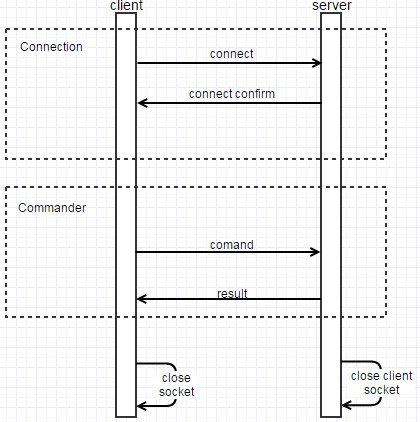
\includegraphics[scale=0.8]{arch}}
				\caption{Архитектура приложения}
				\label{img:arch}
			\end{figure}
\section{Тестирование}
\subsection{Описание тестового стенда и методики тестирования}
\subsection{Тестовый план и результаты тестирования}
1) Тест1: ввод команд без подключения(рис. 2.2)\\
2) Тест2: обработка неверных команд(рис. 2.3)\\
3) Тест3: неправильный путь при загрузке файла на сервер(рис. 2.4)\\
4) Тест4: получение дерева каталогов(рис. 2.5)\\
5) Тест5: получения файла с сервера(рис. 2.6)\\
6) Тест6: отправка файла на сервер(рис. 2.7)\\

Результаты тестирования:\\
			\begin{figure}[h!]
				\center{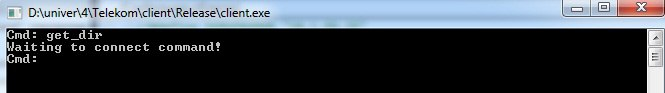
\includegraphics[scale=0.8]{test1}}
				\caption{Ввод команд без подключения}
				\label{img:test1}
			\end{figure}
			\begin{figure}[h!]
				\center{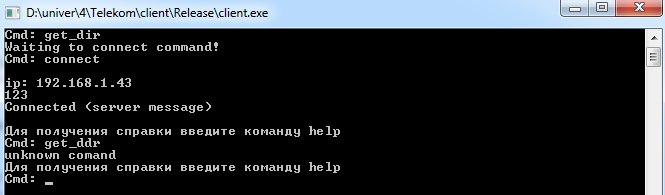
\includegraphics[scale=0.8]{test2}}
				\caption{Обработка неверных команд}
				\label{img:test2}
			\end{figure}
			\begin{figure}[h!]
				\center{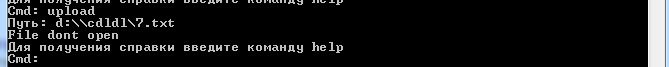
\includegraphics[scale=0.8]{test3}}
				\caption{Неправильный путь при загрузке файла на сервер}
				\label{img:test3}
			\end{figure}
			\begin{figure}[h!]
				\center{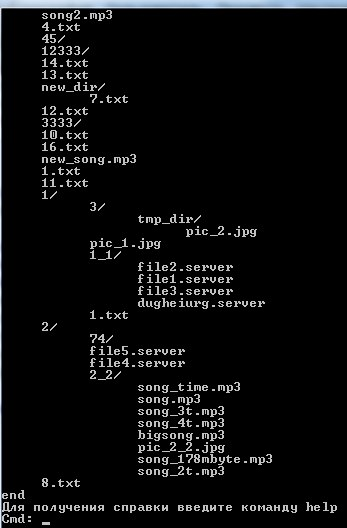
\includegraphics[scale=0.8]{test4}}
				\caption{Получение дерева каталогов}
				\label{img:test4}
			\end{figure}
			\begin{figure}[h!]
				\center{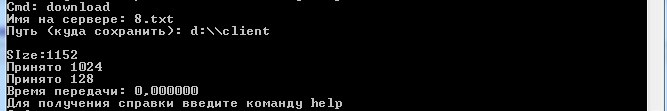
\includegraphics[scale=0.8]{test5}}
				\caption{Получения файла с сервера}
				\label{img:test5}
			\end{figure}
			\begin{figure}[h!]
				\center{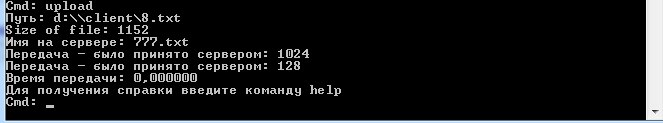
\includegraphics[scale=0.8]{test6}}
				\caption{Отправка файла на сервер}
				\label{img:test6}
			\end{figure}

\chapter{Реализация для работы по протоколу UDP}
\section{Прикладной протокол}
Протоколы команд совпадют с протоколами в реализации TCP, кроме команд upload и download, в которых добавлена проверка на целостность полученного файла. После передачи дополнительная проверка и отправление результата в виде строки "error"/"ок".

\section{Архитектура приложения}
Архитектура приложения относительно реализации TCP немного изменилась. Обработчик команд был обособлен в функцию диспетчера. До диспетчера устанавливается соединение и создание новых сокетов для клиентов.
Архитектура представлена на рисунке 3.1.
\begin{figure}[h!]
				\center{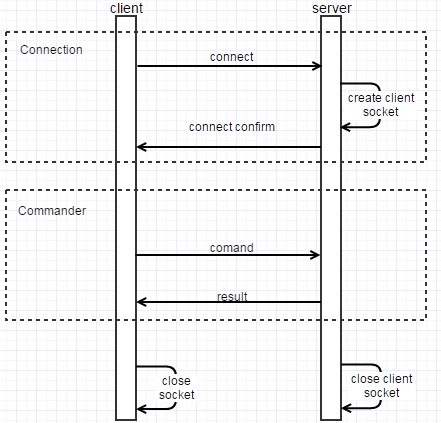
\includegraphics[scale=0.8]{arch2}}
				\caption{Архитектура приложения}
				\label{img:arch2}
			\end{figure}

\section{Тестирование}
\subsection{Описание тестового стенда и методики тестирования}
\subsection{Тестовый план и результаты тестирования}
Тестирование проведено согласно плану тестирования TCP приложений. Результаты совпали.
\\
Тестирование с помощью команды tc.\\
1) Введение задержек командой\\
tc qdisc change dev eth0 root netem delay 100ms 10ms\\
Результат представлен на рис. 3.2.\\
\begin{figure}[h!]
				\center{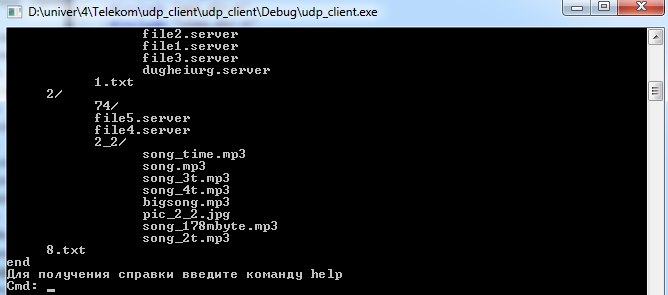
\includegraphics[scale=0.8]{stest1}}
				\caption{Результаты при введении задержек}
				\label{img:stest1}
			\end{figure}
В результате приложение работает нормально, но посылки приходят медленнее.
2)Введение потери пакетов командой \\
tc qdisc change dev eth0 root netem loss 35% \\
Результат представлен на рис. 3.3.\\
\begin{figure}[h!]
				\center{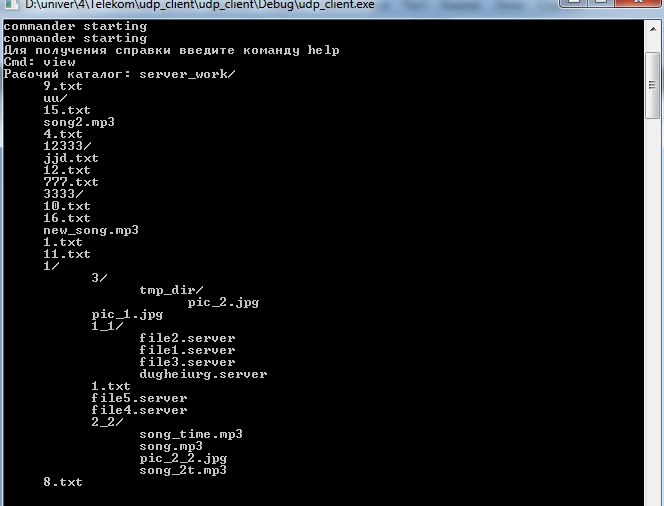
\includegraphics[scale=0.8]{stest3}}
				\caption{Результаты при введении потерь}
				\label{img:stest3}
			\end{figure}
В резульате приложение работает некорректно, т.к. ожидает посылку сервера.\\

3)Введение дупликации пакетов командой \\
tc qdisc change dev eth0 root netem duplicate 35%\\
Результат представлен на рис. 3.4.\\
\begin{figure}[h!]
				\center{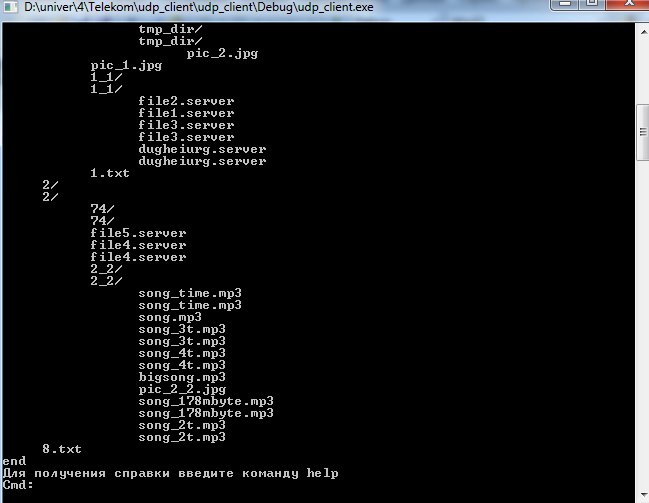
\includegraphics[scale=0.8]{stest4}}
				\caption{Результаты при введении дупликации}
				\label{img:stest4}
			\end{figure}
В резульате приложение работает некорректно, т.к. приходят повторяющиеся данные.\\
\chapter{Тестирование с помощью утилиты valgrind}
Тестирование производилось командой valgrind --leak-check=full ./tcp\_server\\
\begin{lstlisting}
Результаты:
==1441== Memcheck, a memory error detector
==1441== Copyright (C) 2002-2013, and GNU GPLd, by Julian Seward et al.
==1441== Using Valgrind-3.10.0 and LibVEX; rerun with -h for copyright info
==1441== Command: ./tcp_server
==1441== 
Создание сокета
bind
listen
Waiting connections
Connection accepted
==1441== Invalid write of size 4
==1441==    at 0x804A182: main (main.c:63)
==1441==  Address 0x436e028 is 0 bytes inside a block of size 1 alloced
==1441==    at 0x40291CC: malloc (vg_replace_malloc.c:296)
==1441==    by 0x804A175: main (main.c:62)
==1441== 
Handler assigned
==1441== Thread 2:
==1441== Invalid read of size 4
==1441==    at 0x8049A2C: connection_handler (connection_handler.h:16)
==1441==    by 0x41ABEFA: start_thread (pthread_create.c:309)
==1441==    by 0x42AA62D: clone (clone.S:129)
==1441==  Address 0x436e028 is 0 bytes inside a block of size 1 alloced
==1441==    at 0x40291CC: malloc (vg_replace_malloc.c:296)
==1441==    by 0x804A175: main (main.c:62)
==1441== 
^C==1441== 
==1441== HEAP SUMMARY:
==1441==     in use at exit: 145 bytes in 2 blocks
==1441==   total heap usage: 15 allocs, 13 frees, 426,493 bytes allocated
==1441== 
==1441== Thread 1:
==1441== 144 bytes in 1 blocks are possibly lost in loss record 2 of 2
==1441==    at 0x402B0D5: calloc (vg_replace_malloc.c:623)
==1441==    by 0x4010C8E: allocate_dtv (dl-tls.c:296)
==1441==    by 0x40113EB: _dl_allocate_tls (dl-tls.c:460)
==1441==    by 0x41AC72C: allocate_stack (allocatestack.c:589)
==1441==    by 0x41AC72C: pthread_create@@GLIBC_2.1 (pthread_create.c:495)
==1441==    by 0x804A19B: main (main.c:65)
==1441== 
==1441== LEAK SUMMARY:
==1441==    definitely lost: 0 bytes in 0 blocks
==1441==    indirectly lost: 0 bytes in 0 blocks
==1441==      possibly lost: 144 bytes in 1 blocks
==1441==    still reachable: 1 bytes in 1 blocks
==1441==         suppressed: 0 bytes in 0 blocks
==1441== Reachable blocks (those to which a pointer was found) are not shown.
==1441== To see them, rerun with: --leak-check=full --show-leak-kinds=all
==1441== 
==1441== For counts of detected and suppressed errors, rerun with: -v
==1441== ERROR SUMMARY: 3 errors from 3 contexts (suppressed: 0 from 0)
\end{lstlisting}
В итоге 3 ошибки. Результат после исправления:
\begin{lstlisting}
==1502== Memcheck, a memory error detector
==1502== Copyright (C) 2002-2013, and GNU GPLd, by Julian Seward et al.
==1502== Using Valgrind-3.10.0 and LibVEX; rerun with -h for copyright info
==1502== Command: ./tcp_server
==1502== 
Создание сокета
bind
listen
Waiting connections
Connection accepted
Handler assigned
^C==1502== 
==1502== HEAP SUMMARY:
==1502==     in use at exit: 148 bytes in 2 blocks\\
==1502==   total heap usage: 15 allocs, 13 frees, 426,496 bytes allocated\\
==1502== 
==1502== 144 bytes in 1 blocks are possibly lost in loss record 2 of 2\\
==1502==    at 0x402B0D5: calloc (vg_replace_malloc.c:623)\\
==1502==    by 0x4010C8E: allocate_dtv (dl-tls.c:296)\\
==1502==    by 0x40113EB: _dl_allocate_tls (dl-tls.c:460)\\
==1502==    by 0x41AC72C: allocate_stack (allocatestack.c:589)\\
==1502==    by 0x41AC72C: pthread_create@@GLIBC_2.1 (pthread_create.c:495)
==1502==    by 0x804A19B: main (main.c:65)
==1502== 
==1502== LEAK SUMMARY:
==1502==    definitely lost: 0 bytes in 0 blocks
==1502==    indirectly lost: 0 bytes in 0 blocks
==1502==      possibly lost: 144 bytes in 1 blocks
==1502==    still reachable: 4 bytes in 1 blocks
==1502==         suppressed: 0 bytes in 0 blocks
==1502== Reachable blocks (those to which a pointer was found) are not shown.
==1502== To see them, rerun with: --leak-check=full --show-leak-kinds=all
==1502== 
==1502== For counts of detected and suppressed errors, rerun with: -v
==1502== ERROR SUMMARY: 1 errors from 1 contexts (suppressed: 0 from 0)
\end{lstlisting}
Осталась 1 ошибка не влияющая на работу приложения.\\

\chapter{Выводы}
В результате работы были созданы клиентское и серверное приложения для собственного протокола взаимодествия. Было создано две реализации приложения для протоколов TCP и
UDP. Клиентское и серверное приложения были реализованы для двух
разных платформ: ОС Windows и Linux. При реализации использова-
лись стандартные сокеты. Реализации сокетов для использованных ОС
идентичны, портирование программ с одной платформы на другую вы-
полняется достаточно просто.
В результате работы была создана клиент-серверная система загрузки и приема файлов с сервера.
Файлы храянятся в общей папке, клиенты могут создавать, удалять папки, пермещаться по каталогу.
\section{Реализация для TCP}
Протокол TCP удобен для реализации пользовательских приложений,
так как обеспечивает установление соединения и надежную доставку па-
кетов. Протокол обечпечивает стабильное надежное соединение, поэто-
му при реализации своего протокола не требуется волноваться об этом.
Однако, эти дополнительные средства синхронизации требуют больше
времени на доставку, т.е. скорость передачи данных ниже чем в UDP.

\section{Реализация для UDP}
Протокол UDP удобен для реализации приложений, не требующих точ-
ной доставки пакетов. Он позволяет передавать данные с большей скоро-
стью, однако вероятность потери пакета при этом выше, чем в TCP. По-
этому, использовать данный протокол для реализации поставленной за-
дачи не очень удобно. Требуется использовать дополнительные инстру-
менты для подтверждения корректной доставки, т.е. каким-то образом
«симулировать» TCP. Это неудобно и неэффективно.
\chapter*{Приложения}
\section*{Описание среды разработки}
Серерное приложение реализовано на ОС Linux debian 3.16.0 (среда разработки QT Creator 3.5.0), клиентское на ОС Windows 7 (среда разработки Visual Stidio 2010). Срервер запускался на виртуальной машине, соединение через сетвеой мост.

\section*{Листинги}
\subsection*{TCP SERVER}
\subsection*{Основной файл программы main.c}
\begin{lstlisting}
#include <stdio.h>
#include <stdbool.h>
#include <sys/socket.h>
#include <resolv.h>
#include <arpa/inet.h>
#include <errno.h>
#include <string.h>
#include <unistd.h> // для ch_dir
#include<pthread.h>
#include "connection_handler.h"

#define PORT        1234

int main(){
    int sockfd;
    struct sockaddr_in addr, client;
    char dir[MAXBUF] = "/home/user/server/server_work";
    // инициализация рабочей директории
    chdir(dir);

    //Создание сокета TCP
    //AF_INET - стек протоколов TCP/IP, SOXK_STREAM - создание надежного сокета
    //0 - протокол определяется типом сокета

    printf("Создание сокета\n");
    if ( (sockfd = socket(AF_INET, SOCK_STREAM, 0)) < 0 )
    {
        perror("Ошибка создания сокета");
        exit(errno);
    }

    //Задание адреса и порта серверу
    bzero(&addr, sizeof(addr));
    addr.sin_family = AF_INET;
    addr.sin_port = htons(PORT);
    addr.sin_addr.s_addr = INADDR_ANY;

    //Связь сокета с портом
    printf("bind\n");
    if ( bind(sockfd, (struct sockaddr*)&addr, sizeof(addr)) != 0 ){
        perror("ошибка связи сокета");
        exit(errno);
    }


    //включение прослушивания
    // дескриптор сокета, максимальное число очереди
    printf("listen\n");
    if ( listen(sockfd, 1) != 0 ) {
        perror("ошибка включения прослушивания");
        exit(errno);
    }

    puts("Waiting connections");
    int   c = sizeof(struct sockaddr_in);
    int client_sock, *new_sock;
    while( (client_sock = accept(sockfd, (struct sockaddr *)&client, (socklen_t*)&c)) )
    {
        puts("Connection accepted");

        pthread_t sniffer_thread;
        new_sock = malloc(4);
        *new_sock = client_sock;

        if( pthread_create( &sniffer_thread , NULL ,  connection_handler , (void*) new_sock) < 0)
        {
            perror("could not create thread");
            return 1;
        }
        puts("Handler assigned");
    }

    if (client_sock < 0)
    {
        perror("accept failed");
        return 1;
    }
    return 0;
}
\end{lstlisting}
\subsection*{headers}
chdir.h
\begin{lstlisting}
	#ifndef CH_DIR
#define CH_DIR
#include <unistd.h>
#include <string.h>

int ch_dir(char *buffer, int size, int sock){
    bzero(buffer, size);
    recv(sock, buffer, size, 0);
    int i;
    char dir[256] = "/home/user/server/server_work";
    strcat(dir, buffer);
    i = chdir(dir);
    if (i == -1){
        bzero(buffer, size);
        strcpy(buffer, "Недействительный путь!");
        send(sock, buffer, size, 0);

        bzero(buffer, size);
        getcwd(buffer, size);
        send(sock, buffer, size, 0);
    }
    else{
        bzero(buffer, size);
        strcpy(buffer, "succes");
        send(sock, buffer, size, 0);

        bzero(buffer, size);
        getcwd(buffer, size);
        send(sock, buffer, size, 0);
    }
    printf("%s\n", dir);
    return 0;
}

#endif // CH_DIR
\end{lstlisting}
connectionhandler.h
\begin{lstlisting}
#ifndef CONNECTION_HANDLER
#define CONNECTION_HANDLER
#include<pthread.h>
#include "view.h"
#include "get_dir.h"
#include "view_dir.h"
#include "ch_dir.h"
#include "download.h"
#include "mk_dir.h"
#include "rm_dir.h"
#include "upload.h"

void *connection_handler(void *socket_desc)
{
    //socket
    int sock = *(int*)socket_desc;
    char buffer[MAXBUF];
    char dir[MAXBUF] = "/home/user/server/server_work"; // for "view"

    bzero(buffer, MAXBUF);
    strcpy(buffer, "Connected (server message)\n");
    send(sock, buffer, MAXBUF, 0);

    while(1){
         bzero(buffer, MAXBUF);
         recv(sock, buffer, MAXBUF, 0);

        // Проверка команд
         if (strcmp(buffer, "view\r\n") == 0){
             // send(clientfd, "WORK DIRECTORY/\n", 16, 0);
            view(dir, 5, sock);

            bzero( buffer, MAXBUF);
            sprintf( buffer, "%d", 0);
            strcat(buffer, "|");
            strcat(buffer, "d");
             strcat(buffer, "|");
            strcat(buffer, "end");
            send(sock, buffer, MAXBUF, 0);
         }
        if (strcmp(buffer, "view_dir\r\n") == 0){
            chdir("/home/user/server/server_work");
            view_dir(buffer, MAXBUF, sock);

            bzero( buffer, MAXBUF);
            sprintf( buffer, "%d", 0);
            strcat(buffer, "|");
            strcat(buffer, "d");
            strcat(buffer, "|");
             strcat(buffer, "end");
            send(sock, buffer, MAXBUF, 0);
            chdir("/home/user/server/server_work");
        }
        else if (strcmp(buffer,"disconnect")==0){
            //завершение соединения
            close(sock);
            break;
        }
        else if (strcmp(buffer,"get_dir\r\n")==0){
            get_dir(buffer, MAXBUF, sock);
        }
        else if (strcmp(buffer,"ch_dir\r\n")==0){
            ch_dir(buffer, MAXBUF, sock);
        }
        else if (strcmp(buffer,"upload\r\n")==0){
            download(buffer, MAXBUF, sock);
        }
        else if (strcmp(buffer,"download\r\n")==0){
            upload(buffer, MAXBUF, sock);
        }
        else if (strcmp(buffer,"mk_dir\r\n")==0){
            mk_dir(buffer, MAXBUF, sock, S_IRWXU);
        }
        else if (strcmp(buffer,"rm_dir\r\n")==0){
            rm_dir(buffer, MAXBUF, sock);
        }
        else{
                printf("%s", buffer);
                send(sock, "void \n", 5, 0);
         }
    }

    //Free the socket pointer
    free(socket_desc);

    return 0;
}
#endif // THREAD_HANDLER
\end{lstlisting}

download.h
\begin{lstlisting}
#ifndef DOWNLOAD
#define DOWNLOAD
#include <string.h>
#include <stdio.h>
#include <unistd.h>

int download(char *buffer, size_t size, int sock){
    int r;
    int p;
    int i = 0;
    int j = 0;
    int k = 0;
    long int fileSize = 0;
    char send_buf[size], name[size];

    //прием и формирование размера файла
    bzero(buffer, size);
    recv(sock, buffer, size, 0);
    while(buffer[i] != '\0'){
          i++;
          k++;
     }
     for(j=0; j<k; j++){
         p = pow(10,i-1);
         fileSize+=p*((int)buffer[j]-48);
         i--;
     }
    printf("SIze:%d\n", fileSize);


    // прием имени файла
    bzero(buffer, size);
    recv(sock, buffer, size, 0);
    // формирование пути
    bzero(name, size);
    getcwd(name, size);
    strcat(name, "/");
    strcat(name, buffer);
    printf("%s\n", name);

    //формирование пути с именем файла

   FILE* f;
   f = fopen(name, "wb");
   if(f == NULL){
       printf("File dont open\n");
       return -1;
   }

    while(fileSize > 0){
       if(fileSize >=size){
           bzero(buffer, size);
           r = recv(sock, buffer, size, 0);
           fwrite(buffer, 1, size, f); // записываем весь буфер

           // отправка клиенту
           bzero(send_buf, size);
           sprintf(send_buf, "%d",r );
           send(sock, send_buf, size, 0);
       }
       else{
           bzero(buffer, size);
           r = recv(sock, buffer, size, 0);
           fwrite(buffer, 1, fileSize, f); //записываем только сколько надо

           // отправка клиенту
           bzero(send_buf, size);
           sprintf(send_buf, "%d",r );
           send(sock, send_buf, size, 0);
       }
       fileSize -=size;
   }

  /*while(fileSize > 0){
          if(fileSize >=fbuf_size){
              bzero(f_buf, fbuf_size);
              r = recv(sock, f_buf, fbuf_size, 0);
              fwrite(f_buf, 1, size, f); // записываем весь буфер

              // отправка клиенту
              bzero(send_buf, size);
              sprintf(send_buf, "%d",r );
              send(sock, send_buf, size, 0);
          }
          else{
              bzero(f_buf, fbuf_size);
              r = recv(sock, f_buf, fbuf_size, 0);
              fwrite(f_buf, 1, fileSize, f); //записываем только сколько надо

              // отправка клиенту
              bzero(send_buf, size);
              sprintf(send_buf, "%d",r );
              send(sock, send_buf, size, 0);
          }
          fileSize -=fbuf_size;
          printf("now fileSize: %d\n", fileSize);
          printf("now r: %d\n", r);
          sleep(2);
      }*/
   printf("succes!\n");
   fclose(f);
   //free(f_buf);
   return 0;
}

#endif // DOWNLOAD
\end{lstlisting}

getdir.h
\begin{lstlisting}
#ifndef GET_DIR
#define GET_DIR
#include <unistd.h>

int get_dir(char *buffer, size_t size, int clientfd){
    bzero( buffer, size);
    getcwd(buffer, size);
    // отправка клиенту
    send(clientfd, buffer, size, 0);
    return 0;
}

#endif // GET_DIR
\end{lstlisting}

mkdir.h
\begin{lstlisting}
#ifndef MK_DIR
#define MK_DIR
#include <sys/types.h>
#include <sys/stat.h>
#include <string.h>

int mk_dir(char* buffer, int size, int sock, mode_t mode){
    int s;
    bzero(buffer, size);
    recv(sock, buffer, size, 0);
    s = mkdir(buffer, mode);
    if(s == 0){
        bzero(buffer, size);
        strcpy(buffer,"Directory created\n");
        send(sock, buffer, size, 0);
    }
    else{
        bzero(buffer, size);
        strcpy(buffer,"Directory don't created\n");
        send(sock, buffer, size, 0);
    }

    return 0;
}

#endif // MK_DIR
\end{lstlisting}

rmdir.h
\begin{lstlisting}
#ifndef RM_DIR
#define RM_DIR
#include <unistd.h>

int rm_dir(char* buffer, int size, int sock){
    int s;
    bzero(buffer, size);
    recv(sock, buffer, size, 0);
    s = rmdir(buffer);

    if(s == 0){
        bzero(buffer, size);
        strcpy(buffer,"Directory removed\n");
        send(sock, buffer, size, 0);
    }
    else{
        bzero(buffer, size);
        strcpy(buffer,"Directory don't removed\n");
        send(sock, buffer, size, 0);
    }

    return 0;
}
#endif // RM_DIR
\end{lstlisting}

upload.h
\begin{lstlisting}
#ifndef UPLOAD
#define UPLOAD
#include <string.h>
#include <stdio.h>
#include <unistd.h>

int upload(char* buffer, int size, int sock){
    char name[2048], trace[2048];
    int fileSize;
    int message_length;
    FILE* f;

    //прием имени файла
    bzero(name, size);
    recv(sock, name, size, 0);

    //формирование пути открытия файла
    bzero(trace, size);
    getcwd(trace, size);
    strcat(trace, "/");
    strcat(trace, name);

    f = fopen(name, "rb");
    if(f == NULL){
        printf("File dont open\n");
        bzero(buffer, size);
        strcpy(buffer, "false");
        send(sock, buffer, size, 0);
        sleep(0.01);
        return -1;
    }
    else{
        bzero(buffer, size);
        strcpy(buffer, "true");
        send(sock, buffer, size, 0);
        sleep(0.01);
    }


    //отправка размера
    fseek(f, 0, SEEK_END);
    fileSize = ftell(f);
    fseek(f, 0, SEEK_SET);
    printf("Size of file: %d\n", fileSize);
    bzero(buffer, size);
    //strcpy(buffer, (char)fileSize);
    sprintf(buffer, "%d", fileSize);
    send(sock, buffer, size, 0);
    sleep(0.01);

    while(fileSize > 0){
        bzero(buffer, size);
        if(fileSize >=1024){
            message_length = fread(buffer, size, 1, f); // количество

            if(message_length != 0)
                    send(sock, buffer, size, 0);
                    sleep(0.01);
        }
        else{
            message_length = fread(buffer, fileSize, 1, f);

            if(message_length != 0)
                    send(sock, buffer, fileSize, 0);
                    sleep(0.01);
        }
        fileSize -= size;
    }
    fclose(f);

    return 0;
}

#endif // UPLOAD
\end{lstlisting}

view.h
\begin{lstlisting}
#ifndef VIEW_H
#define VIEW_H

#include <string.h>
#include <unistd.h>
#include <dirent.h>
#include <sys/stat.h>
#include <stdlib.h>

#define MAXBUF 1024
void view(char *dir, int depth, int clientfd) {
    //chdir("/home/user/server/server_work");
    // буфер для послыки
    char buffer[MAXBUF];
    DIR *dp;
    struct dirent *entry;
     struct stat statbuf;
     if ((dp = opendir(dir)) == NULL) {
             fprintf(stderr, "cannot open directory: %s\n", dir);
             return;
    }

    chdir(dir);
    while((entry = readdir(dp)) != NULL) {
         lstat(entry->d_name, &statbuf);
         if (S_ISDIR(statbuf.st_mode)) {
             //Находит каталог, но игнорирует . и ..
                if (strcmp(".", entry->d_name) == 0 || strcmp("..", entry->d_name) == 0)
                         continue;

                 bzero( buffer, MAXBUF);
                 sprintf( buffer, "%d", depth);
                 strcat(buffer, "|");
                 strcat(buffer, "d");
                 strcat(buffer, "|");
                 strcat(buffer, entry->d_name);
                 send(clientfd, buffer, MAXBUF, 0);

                int new_depth = depth + 6;
                 // Рекурсивный вызов с новый отступом
                 view(entry->d_name, new_depth, clientfd);
         }
          else {
             bzero( buffer, MAXBUF);
             sprintf( buffer, "%d", depth);
             strcat(buffer, "|");
             strcat(buffer, "f");
             strcat(buffer, "|");
             strcat(buffer, entry->d_name);
             send(clientfd, buffer, MAXBUF, 0);
          }
  }
 chdir("..");
 closedir(dp);
 //chdir("/home/user/server/server_work");
}
#endif // VIEW_H
\end{lstlisting}

viewdir.h\\
\begin{lstlisting}
#ifndef VIEW_DIR
#define VIEW_DIR
#include "view.h"

int view_dir(char *buffer, int buf_size, int clientfd){
    bzero(buffer, buf_size);
    getcwd(buffer, buf_size);
    view(buffer, 5, clientfd);
    return 0;
}
#endif // VIEW_DIR
\end{lstlisting}


\subsection*{TCP client}
\subsection*{headers}
chdir.h
\begin{lstlisting}
#ifndef CHDIR
#define CHDIR
#include <string.h>

int ch_dir(char *buffer, int sock, int size){
	memset(buffer, 0, size);
    strcpy(buffer, "ch_dir\r\n");
    send(sock, buffer, size, 0);

    printf("путь: ");
    memset(buffer, 0, size);
    scanf("%s", buffer);
    send(sock, buffer, size, 0);

    //прием ошибки либо сообщения об успехе
    memset(buffer, 0, size);
    recv(sock, buffer, size, 0);
    if(strcmp(buffer, "succes") != 0)
       printf("Неверный каталог!");

    memset(buffer, 0, size);
    recv(sock, buffer, size, 0);
    printf("Текущий каталог: %s\n", buffer);
    return 0;
}

#endif // CHDIR
\end{lstlisting}

download.h
\begin{lstlisting}
#ifndef DOWNLOAD
#define DOWNLOAD
#include <string.h>
#include <stdio.h>
#include <math.h>
#include <time.h>
#define MAXBUF  1024

int download(char *buffer, size_t size, int sock){
    int r;
    int p;
    int i = 0;
    int j = 0;
    int k = 0;
    int fileSize = 0;
	time_t start_time, finish_time;
    char send_buf[MAXBUF], name[MAXBUF], trace[MAXBUF];

	//отправка команды
	memset(buffer, 0, size);
    strcpy(buffer, "download\r\n");
    send(sock, buffer, size, 0);

	// отправка на сервер имени файла
    printf("Имя на сервере: ");
    memset(name, 0, size);
    scanf("%s",name);
    send(sock, name, size, 0);

	//ожидание подтверждения открытия файла
	memset(buffer, 0, size);
	recv(sock, buffer, size, 0);
	if(strcmp(buffer, "false") == 0){
		printf("Incorrect name - file dont open!\n");
		return -1;
	}

	// где сохранять
	printf("Путь (куда сохранить): ");
    memset(trace, 0, size);
    scanf("%s",trace);
	printf("\n");
	//формирование пути с именем файла
	strcat(trace, "\\");
	strcat(trace, name);

	FILE* f;
	f = fopen(trace, "wb");
	if(f == NULL){
	    printf("File dont create\n");
	    return -1;
	}

    //прием и формирование размера файла
    memset(buffer, 0, size);
    recv(sock, buffer, size, 0);
    while(buffer[i] != '\0'){
          i++;
          k++;
     }
     for(j=0; j<k; j++){
         p = pow(10.0,i-1);
         fileSize+=p*((int)buffer[j]-48);
         i--;
     }
    //printf("size string: %s\n", buffer);
    printf("SIze:%d\n", fileSize);

   
	// запомнить время начала
	start_time = time(NULL);
   while(fileSize > 0){
       if(fileSize >=1024){
           memset(buffer, 0, size);
           r = recv(sock, buffer, size, 0);
           fwrite(buffer, 1, size, f); // записываем весь буфер

           // печать
           memset(send_buf, 0, size);
           printf("Принято %d\n",r );
       }
       else{
           memset(buffer,0, size);
           r = recv(sock, buffer, size, 0);
           fwrite(buffer, 1, fileSize, f); //записываем только сколько надо

           // отправка клиенту
           memset(send_buf,0, size);
           printf("Принято %d\n",r );
       }
       fileSize -=1024;
   }
   // запомнить время завершeния передачи
	finish_time = time(NULL);
   fclose(f);
   printf("Время передачи: %f\n", difftime(finish_time, start_time));
   return 0;
}

#endif // DOWNLOAD
\end{lstlisting}

getdir.h
\begin{lstlisting}
#ifndef GET_DIR
#define GET_DIR
#include <string.h>

int get_dir(char *buffer, int sock, int size){
     memset(buffer, 0, size);
     strcpy(buffer, "get_dir\r\n");
     send(sock, buffer, size, 0);

     // прием
     memset(buffer, 0, size);
     recv(sock, buffer, size,0);
     printf("Текущий каталог: %s\n", buffer);

     return 0;
}
#endif // GET_DIR
\end{lstlisting}

mkdir.h
\begin{lstlisting}
#ifndef MK_DIR
#define MK_DIR
#include <string.h>

int mk_dir(char* buffer, int size, int sock){
    memset(buffer, 0, size);
    strcpy(buffer, "mk_dir\r\n");
    send(sock, buffer, size, 0);

    memset(buffer, 0, size);
    printf("Имя папки: ");
    scanf("%s", buffer);
    send(sock, buffer, size, 0);

    memset(buffer, 0, size);
    recv(sock, buffer, size, 0);
    printf("%s", buffer);
    return 0;
}

#endif // MK_DIR
\end{lstlisting}

rmdir.h
\begin{lstlisting}
#ifndef RM_DIR
#define RM_DIR
#include <string.h>

int rm_dir(char* buffer, int size, int sock){
    memset(buffer, 0, size);
    strcpy(buffer, "rm_dir\r\n");
    send(sock, buffer, size, 0);

    memset(buffer, 0, size);
    printf("Имя папки: ");
    scanf("%s", buffer);
    printf("\n");
    send(sock, buffer, size, 0);

    memset(buffer, 0, size);
    recv(sock, buffer, size, 0);
    printf("%s", buffer);

    return 0;
}

#endif // RM_DIR
\end{lstlisting}

upload.h
\begin{lstlisting}
#ifndef UPLOAD
#define UPLOAD
#include <string.h>
#include <stdio.h>
#include <time.h>
#include <stdlib.h>

int upload(char* buffer, int size, int sock){
    char name[1024];
	//int size = ssize;
	//char *f_buf;//[1024];
    long int fileSize;
    long int message_length;

	time_t start_time, finish_time;
    FILE* f;

	//f_buf = (char*) malloc(fbuf_size);

    printf("Путь: ");
    memset(name, 0, 1024);
    scanf("%s", name);

    f = fopen(name, "rb");
    if(f == NULL){
        printf("File dont open\n");
        return -1;
    }

    memset(buffer, 0, size);
    strcpy(buffer, "upload\r\n");
    send(sock, buffer, size, 0);
	//Sleep(1000);
	   

    //отправка размера
    fseek(f, 0, SEEK_END);
    fileSize = ftell(f);
    fseek(f, 0, SEEK_SET);
    printf("Size of file: %d\n", fileSize);
    memset(buffer, 0, size);
    //strcpy(buffer, (char)fileSize);
    sprintf(buffer, "%d", fileSize);
    send(sock, buffer, size, 0);
	//Sleep(1000);


	// отправка на сервер имени файла
    printf("Имя на сервере: ");
    memset(buffer, 0, size);
    scanf("%s",buffer);
    send(sock, buffer, size, 0);
	//Sleep(1000);

	// запомнить время начала
	start_time = time(NULL);
    
	while(fileSize > 0){
        memset(buffer, 0, size);
        if(fileSize >= size){
            message_length = fread(buffer, size, 1, f); // количество

            if(message_length != 0){
                    send(sock, buffer, size, 0);
					Sleep(1);
			}
            memset(buffer, 0, size);
            recv(sock, buffer, size, 0);
            printf("Передача - было принято сервером: %s\n", buffer);
        }
        else{
            message_length = fread(buffer, fileSize, 1, f);

            if(message_length != 0){
                    send(sock, buffer, fileSize, 0);
					Sleep(1);
			}
            memset(buffer, 0, size);
            recv(sock, buffer, size, 0);
            printf("Передача - было принято сервером: %s\n", buffer);
        }
        fileSize -= size;
    }
	
	
	finish_time = time(NULL);
    fclose(f);
	printf("Время передачи: %f\n", difftime(finish_time, start_time));

    return 0;
}

#endif // UPLOAD
\end{lstlisting}

view.h
\begin{lstlisting}
#ifndef VIEW_H
#define VIEW_H
#include <string.h>
#include <math.h>

int view(char* buffer, int sock, int buf_size){
    printf("Рабочий каталог: server_work/\n");
    memset(buffer, 0, buf_size);
    strcpy(buffer, "view\r\n");
    send(sock, buffer, buf_size, 0);

    while(1){
        int depth;
        int i;
        int j;
        int k;
        memset(buffer, 0, buf_size);
        recv(sock, buffer, buf_size,0);
        if(strcmp(buffer, "0|d|end")==0){
            printf("end\n");
            break;
        }
        else{
            i = 0;
            j = 0;
            k = 0;
            int p=0;
           depth = 0;
           // подсчет количества знаков числа
           while(buffer[i] != '|'){
                 i++;
                 k++;
            }
            for(j=0; j<k; j++){
                p = pow(10.0,i-1);
                depth+=p*((int)buffer[j]-48);
                i--;
            }
            //---------------------------------------------------
            k++; // знак '|'
            if(buffer[k] == 'f')
                p = 0;
            else
                p = 1;
            //----------------------------------------------------
            k++; // знак '|'
            k++;
            // печать пробелов
            for(i=0; i<depth; i++)
                printf(" ");
            // печать названия
            while(buffer[k] != '\0'){
                printf("%c", buffer[k]);
                k++;
            }
            // печать символа папки и перевод строки
            if(p == 1)
                printf("/\n");
            else
                printf("\n");
        }
 }
    return 0;
}

#endif // VIEW_H
\end{lstlisting}

viewdir.h
\begin{lstlisting}
#ifndef view_dir_DIR_H
#define view_dir_DIR_H
#include <string.h>
#include <math.h>

int view_dir(char* buffer, int sock, int size){
    memset(buffer, 0, size);
    strcpy(buffer, "view_dir\r\n");
    send(sock, buffer, size, 0);
    while(1){
        int depth;
        int i;
        int j;
        int k;
        memset(buffer, 0, size);
        recv(sock, buffer, size,0);
        if(strcmp(buffer, "0|d|end")==0){
            printf("end\n");
            break;
        }
        else{
            i = 0;
            j = 0;
            k = 0;
            int p=0;
           depth = 0;
           // подсчет количества знаков числа
           while(buffer[i] != '|'){
                 i++;
                 k++;
            }
            for(j=0; j<k; j++){
                p = pow(10.0,i-1);
                depth+=p*((int)buffer[j]-48);
                i--;
            }
            //---------------------------------------------------
            k++; // знак '|'
            if(buffer[k] == 'f')
                p = 0;
            else
                p = 1;
            //----------------------------------------------------
            k++; // знак '|'
            k++;
            // печать пробелов
            for(i=0; i<depth; i++)
                printf(" ");
            // печать названия
            while(buffer[k] != '\0'){
                printf("%c", buffer[k]);
                k++;
            }
            // печать символа папки и перевод строки
            if(p == 1)
                printf("/\n");
            else
                printf("\n");
        }
 }
    return 0;
}

#endif // view_dir_dir_DIR
\end{lstlisting}
help.h
\begin{lstlisting}
#ifndef HELP
#define HELP
#include <string.h>

int get_help(){
    printf("ch_dir - сменить текущую директорию на сервере\n");
    printf("mk_dir - создать папку в текущей директории\n");
    //printf("download <имя файла> - загрузить файл с сервера\n");
    printf("upload - загрузить файл на сервер из рабочей директории\n");
    printf("view - просмотр дерева каталогов сервера\n");
    //printf("connect <IP> <номер порта> - подключиться к серверу \n");
    printf("disconnect - отключиться от сервера\n");
    return 0;
}

#endif // HELP
\end{lstlisting}

\subsection*{main.c}
\begin{lstlisting}
#define WIN32_LEAN_AND_MEAN  
#include <stdio.h>
#include <conio.h>
#include <string.h>
#include <winsock2.h>
#include <windows.h>
#include <locale.h> 
#include <Ws2tcpip.h>
#pragma comment(lib, "Ws2_32.lib")

#include "view.h"
#include "help.h"
#include "get_dir.h"
#include "view_dir.h"
#include "chdir.h"
#include "upload.h"
#include "rm_dir.h"
#include "mk_dir.h"
#include "echo.h"
#include "download.h"

#define PORT 1234
//#define SERVERADDR "192.168.1.43"
//#define SERVERADDR "10.1.99.25"
#define MAXBUF  1024

  int main()
  {
	char* SERVERADDR;
	SERVERADDR = (char*)malloc(15);
    setlocale(LC_ALL, "Russian");
	char buffer[MAXBUF];
	
	memset(buffer, 0, MAXBUF);
	while(1){
		printf("Cmd: ");
		scanf("%s", buffer);
		if(strcmp("connect", buffer) == 0){
			printf("\nip: ");
			scanf("%s", SERVERADDR);
			break;
		}
		else{
			printf("Waiting to connect command!\n");
			continue;
		}
	}

    //инициализация библиотеки Winsock
    if (WSAStartup(0x202,(WSADATA *)&buffer[0]))
    {
      printf("WSAStart error %d\n",WSAGetLastError());
	  _getch();
      return -1;
    }

    //создание сокета
    SOCKET sock;
    sock=socket(AF_INET,SOCK_STREAM,0);
    if (sock < 0)
    {
      printf("Socket() error %d\n",WSAGetLastError());
	  _getch();
      return -1;
    }

    //установка соединения
    // заполнение структуры sockaddr_in
    // указание адреса и порта сервера
    sockaddr_in dest_addr;
    dest_addr.sin_family=AF_INET;
    dest_addr.sin_port=htons(PORT);
    HOSTENT *hst;

    // преобразование IP адреса из символьного в
    // сетевой формат
    if (inet_addr(SERVERADDR)!=INADDR_NONE)
      dest_addr.sin_addr.s_addr=inet_addr(SERVERADDR);
    else
      // попытка получить IP адрес по доменному
      // имени сервера
      if (hst=gethostbyname(SERVERADDR))
      // hst->h_addr_list содержит не массив адресов,
      // а массив указателей на адреса
      ((unsigned long *)&dest_addr.sin_addr)[0]=
        ((unsigned long **)hst->h_addr_list)[0][0];
      else 
      {
        printf("Invalid address %s\n",SERVERADDR);
        closesocket(sock);
        WSACleanup();
		_getch();
        return -1;
      }
	printf("123\n");
    if (connect(sock,(sockaddr *)&dest_addr,
                sizeof(dest_addr)))
    {
      printf("Connect error %d\n",WSAGetLastError());
	  _getch();
      return -1;
    }
	//-----------------------------------------------
	memset(buffer, 0, MAXBUF);
    recv(sock , buffer , MAXBUF , 0); // прием слова
    puts(buffer);
    printf("Для получения справки введите команду help\n");
    while(1){
		memset(buffer, 0, MAXBUF);
        printf("Cmd: ");
        scanf("%s" , buffer);
        // команды
        if(strcmp(buffer, "view") == 0)
			view_dir(buffer, sock, MAXBUF);
        else if(strcmp(buffer, "view_dir") == 0)
            view_dir(buffer, sock, MAXBUF);
        else if(strcmp(buffer, "help") == 0)
            get_help();
        else if(strcmp(buffer, "get_dir") == 0)
            get_dir(buffer, sock, MAXBUF);
        else if(strcmp(buffer, "ch_dir") == 0)
            ch_dir(buffer, sock, MAXBUF);
        else if(strcmp(buffer, "upload") == 0)
            upload(buffer, MAXBUF, sock);
		else if(strcmp(buffer, "download") == 0)
            download(buffer, MAXBUF, sock);
        else if(strcmp(buffer, "mk_dir") == 0)
            mk_dir(buffer, MAXBUF, sock);
        else if(strcmp(buffer, "rm_dir") == 0)
            rm_dir(buffer, MAXBUF, sock);
		else if(strcmp(buffer, "echo") == 0)
            echo(buffer, sock, MAXBUF);
		else if(strcmp(buffer, "disconnect") == 0){
            send(sock, "disconnect", 10, 0);
			break;
		}
        else
            printf("unknown comand\n");
        printf("Для получения справки введите команду help\n");
    }
	//-----------------------------------------------
	printf("\nExit\n");
    closesocket(sock);
    WSACleanup();
	_getch();
    return 0;
  }
\end{lstlisting}
\subsection*{UDP SERVER}
\subsection*{main.c}
\begin{lstlisting}
#include<stdio.h>
#include<string.h>
#include<stdlib.h>
#include<arpa/inet.h>
#include<sys/socket.h>
#include <pthread.h>
#include "view.h"
#include "get_dir.h"
#include "view_dir.h"
#include "ch_dir.h"
#include "download.h"
#include "mk_dir.h"
#include "rm_dir.h"
#include "upload.h"

#define MAXBUF 1024  //Max length of buffer
#define PORT 1234   //The port on which to listen for incoming data
#define MAXCLIENTS 10
typedef struct {
    int sockfd;
    struct sockaddr_in client;
    int clilen;
} btClient;

int numClients = 0;
btClient clients[MAXCLIENTS];
pthread_mutex_t clientsMutex;

btClient acceptConnection(int sockfd);
void* commander(void* cl);
void errorHandler(int err, char *errfun);
void getNewSocket(int* sockfd, uint16_t* port);

int main(void)
{
    //----------------------------------------------------------------------------------------------------
    pthread_attr_t threadAttr;
    pthread_attr_init(&threadAttr);
    pthread_attr_setdetachstate(&threadAttr, PTHREAD_CREATE_DETACHED);

    //----------init-------------------------------------------------------------------------------------------
    struct sockaddr_in si_me, si_other;

    int sock, i, slen = sizeof(si_other);
     char dir[MAXBUF] = "/home/user/server/server_work";
     // инициализация рабочей директории
     chdir(dir);
    //create a UDP socket
    if ((sock=socket(AF_INET, SOCK_DGRAM, IPPROTO_UDP)) == -1)
    {
        perror("socket");
        exit(-1);
    }
    else
        printf("socket created\n");

    // zero out the structure
    memset((char *) &si_me, 0, sizeof(si_me));

    si_me.sin_family = AF_INET;
    si_me.sin_port = htons(PORT);
    si_me.sin_addr.s_addr = htonl(INADDR_ANY);

    //bind socket to port
    if( bind(sock, (struct sockaddr*)&si_me, sizeof(si_me) ) == -1)
    {
        perror("bind");
        exit(1);
    }
    else
        printf("bind!\n");
    //--------------------------------------------------------------------------------------------------------------------------------------

    while(1) {
            btClient newClient = acceptConnection(sock);
            printf("new client accept\n");
            pthread_t thread;

            if (pthread_create(&thread, NULL, commander, (void*)&newClient) != 0) {
                printf("Error while creating new thread\n");
            }
            else
                printf("New thread created. Client sock = %d\n", newClient.sockfd);
        }
    return 0;
}


void* commander(void* cl) {
    printf("commander starting\n");
    btClient* client = (btClient*) cl;

    printf("set parameters\n");
    struct sockaddr_in si_other = client->client;
    int sock = client->sockfd;
    int slen = client->clilen;
    sendto(sock, "commander starting\n", sizeof("commander starting\n"), 0, (struct sockaddr*) &client->client, client->clilen);

    char buffer[MAXBUF];
   while(1){
    bzero(buffer, MAXBUF);
    int recv_len;
    if ((recv_len = recvfrom(sock, buffer, MAXBUF, 0, (struct sockaddr *) &si_other, &slen)) == -1)
    {
        perror("recvfrom()");
        exit(-1);
    }
    else
     printf("command was received\n");

     char dir[MAXBUF] = "/home/user/server/server_work";
   // Проверка команд
    printf("%s\n", buffer);
    if (strcmp(buffer, "view\r\n") == 0){

       view(dir, 5, sock, si_other, slen);

       bzero( buffer, MAXBUF);
       sprintf( buffer, "%d", 0);
       strcat(buffer, "|");
       strcat(buffer, "d");
        strcat(buffer, "|");
       strcat(buffer, "end");
       //send(sock, buffer, MAXBUF, 0);
       sendto(sock, buffer, MAXBUF, 0, (struct sockaddr*) &si_other, slen);
        chdir("/home/user/server/server_work");
    }
  else if (strcmp(buffer, "view_dir\r\n") == 0){
       chdir("/home/user/server/server_work");
       view_dir(buffer, MAXBUF, sock, si_other, slen);

       bzero( buffer, MAXBUF);
       sprintf( buffer, "%d", 0);
       strcat(buffer, "|");
       strcat(buffer, "d");
       strcat(buffer, "|");
        strcat(buffer, "end");
       //send(sock, buffer, MAXBUF, 0);
        sendto(sock, buffer, MAXBUF, 0, (struct sockaddr*) &si_other, slen);
       chdir("/home/user/server/server_work");
   }
   else if (strcmp(buffer,"disconnect")==0){
       //завершение соединения
       close(sock);
      // break;
   }
   else if (strcmp(buffer,"get_dir\r\n")==0){
       get_dir(buffer, MAXBUF, sock, si_other, slen);
   }
   else if (strcmp(buffer,"ch_dir\r\n")==0){
       ch_dir(buffer, MAXBUF, sock, si_other, slen);
   }
   else if (strcmp(buffer,"upload\r\n")==0){
       download(buffer, MAXBUF, sock, si_other, slen);
   }
   else if (strcmp(buffer,"download\r\n")==0){
       upload(buffer, MAXBUF, sock, si_other, slen);
   }
   else if (strcmp(buffer,"mk_dir\r\n")==0){
       mk_dir(buffer, MAXBUF, sock, S_IRWXU, si_other, slen);
   }
   else if (strcmp(buffer,"rm_dir\r\n")==0){
       rm_dir(buffer, MAXBUF, sock, si_other, slen);
   }
   else{
           printf("%s", buffer);
           //send(sock, "void \n", 5, 0);
           if (sendto(sock, "void\n", 5, 0, (struct sockaddr*) &si_other, slen) == -1)
           {
               perror("sendto()");
               exit(1);
           }
    }
    }
    close(client->sockfd);
    return NULL;
}

btClient acceptConnection(int sockfd) {
    struct sockaddr_in clientaddr; /* client addr */
    int clientlen = sizeof(clientaddr); /* byte size of client's address */
    char buf[MAXBUF];
    int err = 0;

    bzero(buf, MAXBUF);
    err=recvfrom(sockfd, buf, MAXBUF, 0, (struct sockaddr *) &clientaddr, &clientlen);
    errorHandler(err, "ERROR in recvfrom");

    int newsockfd;
    uint16_t newport;
    getNewSocket(&newsockfd, &newport);
    bzero(buf, MAXBUF);
    sprintf(buf, "%d", newport);
    err = sendto(sockfd, buf, strlen(buf), 0, (struct sockaddr *) &clientaddr, clientlen);
    errorHandler(err, "ERROR in sendto");


    // create new socket for this client
    struct sockaddr_in newclientaddr; /* client addr */
    int newclientlen = sizeof(newclientaddr); /* byte size of client's address */
    bzero(buf, MAXBUF);
    err = recvfrom(newsockfd, buf, MAXBUF, 0, (struct sockaddr *) &newclientaddr, &newclientlen);
    printf("%s\n", buf);
    errorHandler(err, "ERROR in recvfrom");

    btClient client;
    client.sockfd = newsockfd;
    client.client = newclientaddr;
    client.clilen = newclientlen;
    return client;
}

int readFrom(btClient* client, char* message, int len) {
    return recvfrom(client->sockfd,
                    message,
                    len,
                    0,
                    (struct sockaddr *) &client->client,
                    &client->clilen);
}

void errorHandler(int err, char *errfun) {
    if (err < 0) {
        printf("Error in function %s\n", errfun);
        exit(1);
    }
}

void getNewSocket(int* sockfd, uint16_t* port) {
    struct sockaddr_in serveraddr;
    int err = 0;
    *sockfd = socket(AF_INET, SOCK_DGRAM, IPPROTO_UDP);
    *port = PORT + (numClients + 1);
    errorHandler(*sockfd, "ERROR opening socket");

    int optval = 1;
    setsockopt(*sockfd, SOL_SOCKET, SO_REUSEADDR, (const void *)&optval , sizeof(int));

    bzero((char *) &serveraddr, sizeof(serveraddr));
    serveraddr.sin_family = AF_INET;
    serveraddr.sin_addr.s_addr = htonl(INADDR_ANY);
    serveraddr.sin_port =htons((unsigned short)*port);

    err = bind(*sockfd, (struct sockaddr *) &serveraddr, sizeof(serveraddr));
    errorHandler(err, "ERROR on binding");
}
\end{lstlisting}
\subsection*{headers}
chdir.h
\begin{lstlisting}
#ifndef CH_DIR
#define CH_DIR
#include <unistd.h>
#include <string.h>

int ch_dir(char *buffer, int size, int sock, struct sockaddr_in si_other, int slen){
    bzero(buffer, size);
    recv(sock, buffer, size, 0);
    int i;
    char dir[256] = "/home/user/server/server_work";
    strcat(dir, buffer);
    i = chdir(dir);
    if (i == -1){
        bzero(buffer, size);
        strcpy(buffer, "Недействительный путь!");
        //send(sock, buffer, size, 0);
        sendto(sock, buffer, MAXBUF, 0, (struct sockaddr*) &si_other, slen);

        bzero(buffer, size);
        getcwd(buffer, size);
        //send(sock, buffer, size, 0);
         sendto(sock, buffer, MAXBUF, 0, (struct sockaddr*) &si_other, slen);
    }
    else{
        bzero(buffer, size);
        strcpy(buffer, "succes");
        //send(sock, buffer, size, 0);
         sendto(sock, buffer, MAXBUF, 0, (struct sockaddr*) &si_other, slen);

        bzero(buffer, size);
        getcwd(buffer, size);
        //send(sock, buffer, size, 0);
         sendto(sock, buffer, MAXBUF, 0, (struct sockaddr*) &si_other, slen);
    }
    printf("%s\n", dir);
    return 0;
}

#endif // CH_DIR
\end{lstlisting}

download.h
\begin{lstlisting}
#ifndef DOWNLOAD
#define DOWNLOAD
#include <string.h>
#include <stdio.h>
#include <unistd.h>

int download(char *buffer, size_t size, int sock, struct sockaddr_in si_other, int slen){
    int r;
    int p;
    int i = 0;
    int j = 0;
    int k = 0;
    long int fileSize = 0;
    char send_buf[size], name[size];

    //прием и формирование размера файла
    bzero(buffer, size);
    //recv(sock, buffer, size, 0);
    recvfrom(sock, buffer, size, 0, (struct sockaddr *) &si_other, &slen);
    while(buffer[i] != '\0'){
          i++;
          k++;
     }
     for(j=0; j<k; j++){
         p = pow(10,i-1);
         fileSize+=p*((int)buffer[j]-48);
         i--;
     }
    printf("SIze:%d\n", fileSize);


    // прием имени файла
    bzero(buffer, size);
    //recv(sock, buffer, size, 0);
    recvfrom(sock, buffer, size, 0, (struct sockaddr *) &si_other, &slen);

    // формирование пути
    bzero(name, size);
    getcwd(name, size);
    strcat(name, "/");
    strcat(name, buffer);
    printf("%s\n", name);

    //формирование пути с именем файла

   FILE* f;
   f = fopen(name, "wb");
   if(f == NULL){
       printf("File dont open\n");
       return -1;
   }

    while(fileSize > 0){
       if(fileSize >=size){
           bzero(buffer, size);
          // r = recv(sock, buffer, size, 0);
           r = recvfrom(sock, buffer, size, 0, (struct sockaddr *) &si_other, &slen);
           fwrite(buffer, 1, size, f); // записываем весь буфер

           // отправка клиенту
           bzero(send_buf, size);
           sprintf(send_buf, "%d",r );
           //send(sock, send_buf, size, 0);
           sendto(sock, send_buf, size, 0, (struct sockaddr*) &si_other, slen);
           sleep(1);
       }
       else{
           bzero(buffer, size);
          // r = recv(sock, buffer, size, 0);
           r = recvfrom(sock, buffer, MAXBUF, 0, (struct sockaddr *) &si_other, &slen);
           fwrite(buffer, 1, fileSize, f); //записываем только сколько надо

           // отправка клиенту
           bzero(send_buf, size);
           sprintf(send_buf, "%d",r );
           //send(sock, send_buf, size, 0);
           sendto(sock, send_buf, size, 0, (struct sockaddr*) &si_other, slen);
           sleep(1);
       }
       fileSize -=size;
   }

   printf("succes!\n");
   fclose(f);
   //free(f_buf);
   return 0;
}

#endif // DOWNLOAD
\end{lstlisting}

getdir.h
\begin{lstlisting}
#ifndef GET_DIR
#define GET_DIR
#include <unistd.h>

int get_dir(char *buffer, size_t size, int clientfd, struct sockaddr_in si_other, int slen){
    bzero( buffer, size);
    getcwd(buffer, size);
    // отправка клиенту
    //send(clientfd, buffer, size, 0);
     sendto(clientfd, buffer, MAXBUF, 0, (struct sockaddr*) &si_other, slen);
    return 0;
}


#endif // GET_DIR
\end{lstlisting}

mkdir.h
\begin{lstlisting}
#ifndef MK_DIR
#define MK_DIR
#include <sys/types.h>
#include <sys/stat.h>
#include <string.h>

int mk_dir(char* buffer, int size, int sock, mode_t mode, struct sockaddr_in si_other, int slen){
    int s;
    bzero(buffer, size);
    //recv(sock, buffer, size, 0);
    recvfrom(sock, buffer, MAXBUF, 0, (struct sockaddr *) &si_other, &slen);
    s = mkdir(buffer, mode);
    if(s == 0){
        bzero(buffer, size);
        strcpy(buffer,"Directory created\n");
        //send(sock, buffer, size, 0);
        sendto(sock, buffer, MAXBUF, 0, (struct sockaddr*) &si_other, slen);
    }
    else{
        bzero(buffer, size);
        strcpy(buffer,"Directory don't created\n");
        //send(sock, buffer, size, 0);
        sendto(sock, buffer, MAXBUF, 0, (struct sockaddr*) &si_other, slen);
    }

    return 0;
}

#endif // MK_DIR
\end{lstlisting}

rmdir.h
\begin{lstlisting}
#ifndef RM_DIR
#define RM_DIR
#include <unistd.h>

int rm_dir(char* buffer, int size, int sock, struct sockaddr_in si_other, int slen){
    int s;
    bzero(buffer, size);
    //recv(sock, buffer, size, 0);
    recvfrom(sock, buffer, MAXBUF, 0, (struct sockaddr *) &si_other, &slen);
    s = rmdir(buffer);

    if(s == 0){
        bzero(buffer, size);
        strcpy(buffer,"Directory removed\n");
        //send(sock, buffer, size, 0);
        sendto(sock, buffer, MAXBUF, 0, (struct sockaddr*) &si_other, slen);
    }
    else{
        bzero(buffer, size);
        strcpy(buffer,"Directory don't removed\n");
        //send(sock, buffer, size, 0);
        sendto(sock, buffer, MAXBUF, 0, (struct sockaddr*) &si_other, slen);
    }

    return 0;
}
#endif // RM_DIR
\end{lstlisting}

upload.h
\begin{lstlisting}
#ifndef UPLOAD
#define UPLOAD
#include <string.h>
#include <stdio.h>
#include <unistd.h>

int upload(char* buffer, int size, int sock, struct sockaddr_in si_other, int slen){
    char name[2048], trace[2048];
    int fileSize;
    int message_length;
    FILE* f;

    //прием имени файла
    bzero(name, size);
    //recv(sock, name, size, 0);
    int r = recvfrom(sock, name, size, 0, (struct sockaddr *) &si_other, &slen);
    printf("%d\n", r);

    //формирование пути открытия файла
    bzero(trace, size);
    getcwd(trace, size);
    strcat(trace, "/");
    strcat(trace, name);
    printf("%s\n", trace);

    f = fopen(name, "rb");
    if(f == NULL){
        printf("File dont open\n");
        bzero(buffer, size);
        strcpy(buffer, "false");
        //send(sock, buffer, size, 0);
        sendto(sock, buffer, size, 0, (struct sockaddr*) &si_other, slen);
        sleep(1);
        return -1;
    }
    else{
        bzero(buffer, size);
        strcpy(buffer, "true");
        //send(sock, buffer, size, 0);
        sendto(sock, buffer, size, 0, (struct sockaddr*) &si_other, slen);
        sleep(1);
    }


    //отправка размера
    fseek(f, 0, SEEK_END);
    fileSize = ftell(f);
    fseek(f, 0, SEEK_SET);
    printf("Size of file: %d\n", fileSize);
    bzero(buffer, size);
    //strcpy(buffer, (char)fileSize);
    sprintf(buffer, "%d", fileSize);
    //send(sock, buffer, size, 0);
    sendto(sock, buffer, size, 0, (struct sockaddr*) &si_other, slen);
    sleep(1);

    while(fileSize > 0){
        bzero(buffer, size);
        if(fileSize >=1024){
            message_length = fread(buffer, size, 1, f); // количество

            if(message_length != 0)
                    //send(sock, buffer, size, 0);
                    sendto(sock, buffer, size, 0, (struct sockaddr*) &si_other, slen);
                    sleep(1);
        }
        else{
            message_length = fread(buffer, fileSize, 1, f);

            if(message_length != 0)
                    //send(sock, buffer, fileSize, 0);
                    sendto(sock, buffer, fileSize, 0, (struct sockaddr*) &si_other, slen);
                    sleep(1);
        }
        fileSize -= size;
    }
    fclose(f);

    return 0;
}

#endif // UPLOAD
\end{lstlisting}

view.h
\begin{lstlisting}
	#ifndef VIEW_H
#define VIEW_H

#include <string.h>
#include <unistd.h>
#include <dirent.h>
#include <sys/stat.h>
#include <stdlib.h>

#define MAXBUF 1024
void view(char *dir, int depth, int clientfd, struct sockaddr_in si_other, int slen) {

    //chdir("/home/user/server/server_work");
    // буфер для посылки
    char buffer[MAXBUF];
    DIR *dp;
    struct dirent *entry;
     struct stat statbuf;
     if ((dp = opendir(dir)) == NULL) {
             fprintf(stderr, "cannot open directory: %s\n", dir);
             return;
    }

    chdir(dir);
    while((entry = readdir(dp)) != NULL) {
         lstat(entry->d_name, &statbuf);
         if (S_ISDIR(statbuf.st_mode)) {
             //Находит каталог, но игнорирует . и ..
                if (strcmp(".", entry->d_name) == 0 || strcmp("..", entry->d_name) == 0)
                         continue;

                 bzero( buffer, MAXBUF);
                 sprintf( buffer, "%d", depth);
                 strcat(buffer, "|");
                 strcat(buffer, "d");
                 strcat(buffer, "|");
                 strcat(buffer, entry->d_name);
                 //send(clientfd, buffer, MAXBUF, 0);
                 sendto(clientfd, buffer, MAXBUF, 0, (struct sockaddr*) &si_other, slen);

                int new_depth = depth + 6;
                 // Рекурсивный вызов с новый отступом
                 view(entry->d_name, new_depth, clientfd, si_other, slen);
         }
          else {
             bzero( buffer, MAXBUF);
             sprintf( buffer, "%d", depth);
             strcat(buffer, "|");
             strcat(buffer, "f");
             strcat(buffer, "|");
             strcat(buffer, entry->d_name);
             //send(clientfd, buffer, MAXBUF, 0);
             sendto(clientfd, buffer, MAXBUF, 0, (struct sockaddr*) &si_other, slen);
          }
  }
 chdir("..");
 closedir(dp);
 //chdir("/home/user/server/server_work");
}
#endif // VIEW_H
\end{lstlisting}

viewdir.h
\begin{lstlisting}

#ifndef VIEW_DIR
#define VIEW_DIR
#include "view.h"

int view_dir(char *buffer, int buf_size, int sock, struct sockaddr_in si_other, int slen){
    bzero(buffer, buf_size);
    getcwd(buffer, buf_size);
    view(buffer, 5, sock, si_other, slen);
    return 0;
}

#endif // VIEW_DIR
\end{lstlisting}


\subsection*{UDP CLIENT}
\subsection*{main.c}
\begin{lstlisting}
#define WIN32_LEAN_AND_MEAN  
#include <stdio.h>
#include <conio.h>
#include <string.h>
#include <winsock2.h>
#include <windows.h>
#include <locale.h> 
#include <Ws2tcpip.h>
#pragma comment(lib, "Ws2_32.lib")

#include "view.h"
#include "help.h"
#include "get_dir.h"
#include "view_dir.h"
#include "chdir.h"
#include "upload.h"
#include "rm_dir.h"
#include "mk_dir.h"
#include "echo.h"
#include "download.h"

#define PORT 1234
//#define SERVERADDR "192.168.1.43"
//#define SERVERADDR "10.1.99.25"
#define SERVERADDR "10.1.99.119"
#define MAXBUF  1024

  int main()
  {
	//char* SERVERADDR;
	//SERVERADDR = (char*)malloc(15);
    setlocale(LC_ALL, "Russian");
	char buffer[MAXBUF];
	
	memset(buffer, 0, MAXBUF);
	/*while(1){
		printf("Cmd: ");
		scanf("%s", buffer);
		if(strcmp("connect", buffer) == 0){
			printf("\nip: ");
			scanf("%s", SERVERADDR);
			break;
		}
		else{
			printf("Waiting to connect command!\n");
			continue;
		}
	}*/

    // Шаг 1 - иницилизация библиотеки Winsocks
    if (WSAStartup(0x202,(WSADATA *)&buffer[0]))
    {
      printf("WSAStartup error: %d\n",
             WSAGetLastError());
      return -1;
    }

    // Шаг 2 - открытие сокета
    SOCKET sock=socket(AF_INET, SOCK_DGRAM, 0);
    if (sock==INVALID_SOCKET)
    {
      printf("socket() error: %d\n",WSAGetLastError());
      WSACleanup();
      return -1;
    }

    // Шаг 3 - обмен сообщений с сервером
    HOSTENT *hst;
    sockaddr_in dest_addr;
	int slen = sizeof(dest_addr);

    dest_addr.sin_family=AF_INET;
    dest_addr.sin_port=htons(PORT);

    // определение IP-адреса узла
    if (inet_addr(SERVERADDR))
      dest_addr.sin_addr.s_addr=inet_addr(SERVERADDR);
    else
      if (hst=gethostbyname(SERVERADDR))
        dest_addr.sin_addr.s_addr=((unsigned long **)
              hst->h_addr_list)[0][0];
    else
      {
        printf("Unknown host: %d\n",WSAGetLastError());
        closesocket(sock);
        WSACleanup();
        return -1;
      }
	//----------------------------------------------------
	 //первая отправка
	  printf("Идет первая отправка...\n");
	  sendto(sock, "123", 3, 0, (struct sockaddr*) &dest_addr, slen);
	  //прием порта
	  memset(buffer, 0, MAXBUF);
	  int r;
	  if( (r=recvfrom(sock, buffer, MAXBUF, 0, (struct sockaddr *) &dest_addr, &slen)) != -1 ){
		printf("Порт принят!\n");
	  }
	//закрытие старого сокета
	closesocket(sock);
    WSACleanup();
	printf("Закрыт старый сокет\n");

	int newport = atoi(buffer);
	printf("Установлен новый порт\n");

	WSADATA wsa2;
	if (WSAStartup(MAKEWORD(2, 2), &wsa2) != 0) {
		exit(EXIT_FAILURE);
	}

	struct sockaddr_in new_si_other;
	int sockfd, new_slen = sizeof(new_si_other);

	//новый сокет
	if ((sockfd = socket(AF_INET, SOCK_DGRAM, IPPROTO_UDP)) == SOCKET_ERROR) {
		exit(EXIT_FAILURE);
	}
	else
		printf("Создан новый сокет\n");

	//установка параметров
	memset((char *)&new_si_other, 0, new_slen);
	new_si_other.sin_family = AF_INET;
	new_si_other.sin_port = htons(newport);
	new_si_other.sin_addr.S_un.S_addr = inet_addr(SERVERADDR);
	printf("Установлены параметры\n");

	//новая отправка
	printf("Новая отправка\n");
	if((r=sendto(sockfd, "345", 3, 0, (struct sockaddr *) &new_si_other, new_slen)) != -1)
		printf("Успешная новая отправка\n");
	else
		printf("Новая отправка не удалась\n");

	// ожилание приема сообщение о работе диспетчера
	memset(buffer, 0, MAXBUF);
	if ((r=recvfrom(sockfd, buffer, MAXBUF, 0, (struct sockaddr *) &new_si_other, &new_slen)) != -1){
		printf("Диспетчер работает\n");
		printf("%s", buffer);
	}
	else
		printf("Диспетчер не работает\n");
	printf("%s", buffer);
	//----------------------------------------------------
    printf("Для получения справки введите команду help\n");
    while(1){
		memset(buffer, 0, MAXBUF);
        printf("Cmd: ");
        scanf("%s" , buffer);
        // команды
        if(strcmp(buffer, "view") == 0){
			view(buffer, sockfd, MAXBUF, new_si_other, new_slen);
		}
        else if(strcmp(buffer, "view_dir") == 0)
            view_dir(buffer, sockfd, MAXBUF, new_si_other, new_slen);
        else if(strcmp(buffer, "help") == 0)
            get_help();
        else if(strcmp(buffer, "get_dir") == 0)
            get_dir(buffer, sockfd, MAXBUF, new_si_other, new_slen);
        else if(strcmp(buffer, "ch_dir") == 0)
            ch_dir(buffer, sockfd, MAXBUF, dest_addr, new_slen);
        else if(strcmp(buffer, "upload") == 0)
            upload(buffer, MAXBUF, sockfd, new_si_other, new_slen);
		else if(strcmp(buffer, "download") == 0)
            download(buffer, MAXBUF, sockfd, new_si_other, new_slen);
        else if(strcmp(buffer, "mk_dir") == 0)
            mk_dir(buffer, MAXBUF, sockfd, new_si_other, new_slen);
        else if(strcmp(buffer, "rm_dir") == 0)
            rm_dir(buffer, MAXBUF, sockfd, new_si_other, new_slen);
		else if(strcmp(buffer, "echo") == 0)
            echo(buffer, sockfd, MAXBUF, new_si_other, new_slen);
		else if(strcmp(buffer, "disconnect") == 0){
            sendto(sockfd, "disconnect", 10, 0, (struct sockaddr*) &new_si_other, new_slen);
			break;
		}
        else
            printf("unknown comand\n");
        printf("Для получения справки введите команду help\n");
    }
	//-----------------------------------------------
	printf("\nExit\n");
    closesocket(sockfd);
    WSACleanup();
	_getch();
    return 0;
  }
\end{lstlisting}
\subsection*{headers}
chdir.h
\begin{lstlisting}
#ifndef CHDIR
#define CHDIR
#include <string.h>

int ch_dir(char *buffer, int sock, int size, struct sockaddr_in dest_addr, int slen){
	memset(buffer, 0, size);
    strcpy(buffer, "ch_dir\r\n");
    //send(sock, buffer, size, 0);
	sendto(sock, buffer, size, 0, (struct sockaddr*) &dest_addr, slen);

    printf("путь: ");
    memset(buffer, 0, size);
    scanf("%s", buffer);
    //send(sock, buffer, size, 0);
	sendto(sock, buffer, size, 0, (struct sockaddr*) &dest_addr, slen);

    //прием ошибки либо сообщения об успехе
    memset(buffer, 0, size);
    //recv(sock, buffer, size, 0);
	recvfrom(sock, buffer, size, 0, (struct sockaddr *) &dest_addr, &slen);
    if(strcmp(buffer, "succes") != 0)
       printf("Неверный каталог!");

    memset(buffer, 0, size);
    //recv(sock, buffer, size, 0);
	recvfrom(sock, buffer, size, 0, (struct sockaddr *) &dest_addr, &slen);
    printf("Текущий каталог: %s\n", buffer);
    return 0;
}

#endif // CHDIR
\end{lstlisting}

download.h
\begin{lstlisting}
#ifndef DOWNLOAD
#define DOWNLOAD
#include <string.h>
#include <stdio.h>
#include <math.h>
#include <sys/stat.h>
#include <time.h>
#define MAXBUF  1024

int download(char *buffer, size_t size, int sock, struct sockaddr_in dest_addr, int slen){
    int r;
    int p;
    int i = 0;
    int j = 0;
    int k = 0;
    int fileSize = 0;
	time_t start_time, finish_time;
    char send_buf[MAXBUF], name[MAXBUF], trace[MAXBUF];

	//отправка команды
	memset(buffer, 0, size);
    strcpy(buffer, "download\r\n");
    //send(sock, buffer, size, 0);
	sendto(sock, buffer, size, 0, (struct sockaddr*) &dest_addr, slen);

	// отправка на сервер имени файла
    printf("Имя на сервере: ");
    memset(name, 0, size);
    scanf("%s",name);
    //send(sock, name, size, 0);
	sendto(sock, name, size, 0, (struct sockaddr*) &dest_addr, slen);

	//ожидание подтверждения открытия файла
	memset(buffer, 0, size);
	//recv(sock, buffer, size, 0);
	recvfrom(sock, buffer, size, 0, (struct sockaddr *) &dest_addr, &slen);
	if(strcmp(buffer, "false") == 0){
		printf("Incorrect name - file dont open!\n");
		return -1;
	}

	// где сохранять
	printf("Путь (куда сохранить): ");
    memset(trace, 0, size);
    scanf("%s",trace);
	printf("\n");
	//формирование пути с именем файла
	strcat(trace, "\\");
	strcat(trace, name);

	FILE* f;
	f = fopen(trace, "wb");
	if(f == NULL){
	    printf("File dont create\n");
	    return -1;
	}

    //прием и формирование размера файла
    memset(buffer, 0, size);
    //recv(sock, buffer, size, 0);
	recvfrom(sock, buffer, size, 0, (struct sockaddr *) &dest_addr, &slen);
    while(buffer[i] != '\0'){
          i++;
          k++;
     }
     for(j=0; j<k; j++){
         p = pow(10.0,i-1);
         fileSize+=p*((int)buffer[j]-48);
         i--;
     }
    //printf("size string: %s\n", buffer);
    printf("SIze:%d\n", fileSize);

   int fileSize_copy = fileSize;
	// запомнить время начала
	start_time = time(NULL);
   while(fileSize > 0){
       if(fileSize >=1024){
           memset(buffer, 0, size);
           //r = recv(sock, buffer, size, 0);
		   r = recvfrom(sock, buffer, size, 0, (struct sockaddr *) &dest_addr, &slen);
           fwrite(buffer, 1, size, f); // записываем весь буфер

           // печать
           memset(send_buf, 0, size);
           printf("Принято %d\n",r );
       }
       else{
           memset(buffer,0, size);
           //r = recv(sock, buffer, size, 0);
		   r = recvfrom(sock, buffer, size, 0, (struct sockaddr *) &dest_addr, &slen);
           fwrite(buffer, 1, fileSize, f); //записываем только сколько надо

           // отправка клиенту
           memset(send_buf,0, size);
           printf("Принято %d\n",r );
       }
       fileSize -=1024;
   }
   // запомнить время завершeния передачи
	finish_time = time(NULL);
   fclose(f);
   //проверка
   struct stat fi;
   stat(trace,&fi);
   if(fileSize > fi.st_size)
	   printf("Файл получен с ошибкой! Осуществите повторный прием!\n");
   printf("Время передачи: %f\n", difftime(finish_time, start_time));
   return 0;
}

#endif // DOWNLOAD
\end{lstlisting}

getdir.h
\begin{lstlisting}
#ifndef GET_DIR
#define GET_DIR
#include <string.h>

int get_dir(char *buffer, int sock, int size, struct sockaddr_in dest_addr, int slen){
     memset(buffer, 0, size);
     strcpy(buffer, "get_dir\r\n");
     //send(sock, buffer, size, 0);
	 sendto(sock, buffer, size, 0, (struct sockaddr*) &dest_addr, slen);

     // прием
     memset(buffer, 0, size);
     //recv(sock, buffer, size,0);
	 recvfrom(sock, buffer, size, 0, (struct sockaddr *) &dest_addr, &slen);
     printf("Текущий каталог: %s\n", buffer);

     return 0;
}
#endif // GET_DIR
\end{lstlisting}

mkdir.h
\begin{lstlisting}
#ifndef MK_DIR
#define MK_DIR
#include <string.h>

int mk_dir(char* buffer, int size, int sock, struct sockaddr_in dest_addr, int slen){
    memset(buffer, 0, size);
    strcpy(buffer, "mk_dir\r\n");
    //send(sock, buffer, size, 0);
	sendto(sock, buffer, size, 0, (struct sockaddr*) &dest_addr, slen);

    memset(buffer, 0, size);
    printf("Имя папки: ");
    scanf("%s", buffer);
    //send(sock, buffer, size, 0);
	sendto(sock, buffer, size, 0, (struct sockaddr*) &dest_addr, slen);

    memset(buffer, 0, size);
    //recv(sock, buffer, size, 0);
	recvfrom(sock, buffer, size, 0, (struct sockaddr *) &dest_addr, &slen);
    printf("%s", buffer);
    return 0;
}

#endif // MK_DIR
\end{lstlisting}

rmdir.h
\begin{lstlisting}
#ifndef RM_DIR
#define RM_DIR
#include <string.h>

int rm_dir(char* buffer, int size, int sock, struct sockaddr_in dest_addr, int slen){
    memset(buffer, 0, size);
    strcpy(buffer, "rm_dir\r\n");
    //send(sock, buffer, size, 0);
	sendto(sock, buffer, size, 0, (struct sockaddr*) &dest_addr, slen);

    memset(buffer, 0, size);
    printf("Имя папки: ");
    scanf("%s", buffer);
    printf("\n");
    //send(sock, buffer, size, 0);
	sendto(sock, buffer, size, 0, (struct sockaddr*) &dest_addr, slen);

    memset(buffer, 0, size);
    //recv(sock, buffer, size, 0);
	recvfrom(sock, buffer, size, 0, (struct sockaddr *) &dest_addr, &slen);
    printf("%s", buffer);

    return 0;
}

#endif // RM_DIR
\end{lstlisting}

upload.h
\begin{lstlisting}
#ifndef UPLOAD
#define UPLOAD
#include <string.h>
#include <stdio.h>
#include <time.h>
#include <stdlib.h>

int upload(char* buffer, int size, int sock, struct sockaddr_in dest_addr, int slen){
    char name[1024];
	//int size = ssize;
	//char *f_buf;//[1024];
    long int fileSize;
    long int message_length;

	time_t start_time, finish_time;
    FILE* f;

	//f_buf = (char*) malloc(fbuf_size);

    printf("Путь: ");
    memset(name, 0, 1024);
    scanf("%s", name);

    f = fopen(name, "rb");
    if(f == NULL){
        printf("File dont open\n");
        return -1;
    }

    memset(buffer, 0, size);
    strcpy(buffer, "upload\r\n");
    //send(sock, buffer, size, 0);
	sendto(sock, buffer, size, 0, (struct sockaddr*) &dest_addr, slen);
	Sleep(0.01);
	   

    //отправка размера
    fseek(f, 0, SEEK_END);
    fileSize = ftell(f);
    fseek(f, 0, SEEK_SET);
    printf("Size of file: %d\n", fileSize);
    memset(buffer, 0, size);
    //strcpy(buffer, (char)fileSize);
    sprintf(buffer, "%d", fileSize);
    //send(sock, buffer, size, 0);
	sendto(sock, buffer, size, 0, (struct sockaddr*) &dest_addr, slen);
	Sleep(1);


	// отправка на сервер имени файла
    printf("Имя на сервере: ");
    memset(buffer, 0, size);
    scanf("%s",buffer);
    //send(sock, buffer, size, 0);
	sendto(sock, buffer, size, 0, (struct sockaddr*) &dest_addr, slen);
	Sleep(0.01);

	// запомнить время начала
	start_time = time(NULL);
    
	while(fileSize > 0){
        memset(buffer, 0, size);
        if(fileSize >= size){
			memset(buffer, 0, size);
            message_length = fread(buffer, size, 1, f); // количество

            if(message_length != 0){
                    //send(sock, buffer, size, 0);
					sendto(sock, buffer, size, 0, (struct sockaddr*) &dest_addr, slen);
					Sleep(0.01);
			}
            memset(buffer, 0, size);
            //recv(sock, buffer, size, 0);
			recvfrom(sock, buffer, size, 0, (struct sockaddr *) &dest_addr, &slen);
            printf("Передача - было принято сервером: %s\n", buffer);
        }
        else{
			memset(buffer, 0, size);
            message_length = fread(buffer, fileSize, 1, f);

            if(message_length != 0){
                    //send(sock, buffer, fileSize, 0);
					sendto(sock, buffer, fileSize, 0, (struct sockaddr*) &dest_addr, slen);
					Sleep(0.01);
			}
            memset(buffer, 0, size);
            //recv(sock, buffer, size, 0);
			recvfrom(sock, buffer, size, 0, (struct sockaddr *) &dest_addr, &slen);
            printf("Передача - было принято сервером: %s\n", buffer);
        }
        fileSize -= size;
    }
	
	finish_time = time(NULL);
    fclose(f);
	printf("Время передачи: %f\n", difftime(finish_time, start_time));

    return 0;
}

#endif // UPLOAD
\end{lstlisting}

view.h
\begin{lstlisting}
#ifndef VIEW_H
#define VIEW_H
#include <string.h>
#include <math.h>

int view(char* buffer, int sock, int buf_size, struct sockaddr_in dest_addr, int slen){
    printf("Рабочий каталог: server_work/\n");
    memset(buffer, 0, buf_size);
    strcpy(buffer, "view\r\n");
    //send(sock, buffer, buf_size, 0);
	sendto(sock, buffer, buf_size, 0, (struct sockaddr*) &dest_addr, slen);

    while(1){
        int depth;
        int i;
        int j;
        int k;
        memset(buffer, 0, buf_size);
        //recv(sock, buffer, buf_size,0);
		recvfrom(sock, buffer, buf_size, 0, (struct sockaddr *) &dest_addr, &slen);
        if(strcmp(buffer, "0|d|end")==0){
            printf("end\n");
            break;
        }
        else{
            i = 0;
            j = 0;
            k = 0;
            int p=0;
           depth = 0;
           // подсчет количества знаков числа
           while(buffer[i] != '|'){
                 i++;
                 k++;
            }
            for(j=0; j<k; j++){
                p = pow(10.0,i-1);
                depth+=p*((int)buffer[j]-48);
                i--;
            }
            //---------------------------------------------------
            k++; // знак '|'
            if(buffer[k] == 'f')
                p = 0;
            else
                p = 1;
            //----------------------------------------------------
            k++; // знак '|'
            k++;
            // печать пробелов
            for(i=0; i<depth; i++)
                printf(" ");
            // печать названия
            while(buffer[k] != '\0'){
                printf("%c", buffer[k]);
                k++;
            }
            // печать символа папки и перевод строки
            if(p == 1)
                printf("/\n");
            else
                printf("\n");
        }
 }
    return 0;
}

#endif // VIEW_H
\end{lstlisting}

viewdir.h
\begin{lstlisting}
#ifndef view_dir_DIR_H
#define view_dir_DIR_H
#include <string.h>
#include <math.h>

int view_dir(char* buffer, int sock, int size, struct sockaddr_in dest_addr, int slen){
    memset(buffer, 0, size);
    strcpy(buffer, "view_dir\r\n");
    //send(sock, buffer, size, 0);
	sendto(sock, buffer, size, 0, (struct sockaddr*) &dest_addr, slen);
    while(1){
        int depth;
        int i;
        int j;
        int k;
        memset(buffer, 0, size);
        //recv(sock, buffer, size,0);
		recvfrom(sock, buffer, size, 0, (struct sockaddr *) &dest_addr, &slen);
        if(strcmp(buffer, "0|d|end")==0){
            printf("end\n");
            break;
        }
        else{
            i = 0;
            j = 0;
            k = 0;
            int p=0;
           depth = 0;
           // подсчет количества знаков числа
           while(buffer[i] != '|'){
                 i++;
                 k++;
            }
            for(j=0; j<k; j++){
                p = pow(10.0,i-1);
                depth+=p*((int)buffer[j]-48);
                i--;
            }
            //---------------------------------------------------
            k++; // знак '|'
            if(buffer[k] == 'f')
                p = 0;
            else
                p = 1;
            //----------------------------------------------------
            k++; // знак '|'
            k++;
            // печать пробелов
            for(i=0; i<depth; i++)
                printf(" ");
            // печать названия
            while(buffer[k] != '\0'){
                printf("%c", buffer[k]);
                k++;
            }
            // печать символа папки и перевод строки
            if(p == 1)
                printf("/\n");
            else
                printf("\n");
        }
 }
    return 0;
}

#endif // view_dir_dir_DIR
\end{lstlisting}
help.h
\begin{lstlisting}
#ifndef HELP
#define HELP
#include <string.h>

int get_help(){
    printf("ch_dir - сменить текущую директорию на сервере\n");
    printf("mk_dir - создать папку в текущей директории\n");
    //printf("download <имя файла> - загрузить файл с сервера\n");
    printf("upload - загрузить файл на сервер из рабочей директории\n");
    printf("view - просмотр дерева каталогов сервера\n");
    //printf("connect <IP> <номер порта> - подключиться к серверу \n");
    printf("disconnect - отключиться от сервера\n");
    return 0;
}

#endif // HELP
\end{lstlisting}
%\lstinputlisting[]
%{/home/user/workspace/tcp_server/main.c}
%\subsection*{Файл сборки Makefile}
%\lstinputlisting[language=make,label={Makefile}]
%{/home/user/workspace/tcp_server/Makefile}

\end{document}
